\documentclass{article}

\usepackage{times}
%\usepackage{uist}
%\usepackage[config, font=small, labelfont={sf,bf}, textfont=sf]{caption,subfig}
\usepackage{setspace}
\doublespace
\usepackage[config, font=small, labelfont={sf,bf}, textfont=sf]{caption}
\usepackage{subfig}
\usepackage{graphicx}

\begin{document}

% --- Copyright notice ---
%\conferenceinfo{UIST'11}{October 16-19, 2011, Santa Barbara, CA, USA}
%\CopyrightYear{2011}
%\crdata{978-1-4503-0716-1/11/10}

% Uncomment the following line to hide the copyright notice
\toappear{}
% ------------------------

\bibliographystyle{plain}

\title{Sketch It, Make It: Freehand Drawing for Precise Rapid Fabrication}

\author{
\parbox[t]{9cm}{\centering
	     {\em Author One}\\
	     Institution Name\\
             City, ST, USA\\
	     user@institution.net}
\parbox[t]{9cm}{\centering
	     {\em Author Two}\\
	     Institution Name\\
             City, ST, USA\\
	     user@institution.net}
}

\maketitle

% TODO: change this
\abstract Abstract goes here. 

\classification{I.3.5 [Computational Geometry and Object Modeling]: Modeling packages}

% TODO: change this
\terms{Design, Human Factors}

\keywords{sketching, rapid fabrication, design tools, constraints}

\tolerance=400 % prevent words from sticking out in the margin

%% \begin{figure}[tb]
%% \vspace{1.9in}
%% \caption{A figure caption.  It is set in 9 point Helvetica type, with a
%% 0.5 cm wider margin on both left and right sides.} 
%% \label{fig-example}
%% \end{figure}

\section{INTRODUCTION}

A growing community of self-described \textit{Makers} design and build
many kinds of physical things~\cite{gershenfeld-fab}. Some are
electronic gizmos, while others are made entirely from traditional
materials. These ``new makers''~\cite{gross-new-makers} are empowered
by rapid fabrication machines like 3D printers and laser cutters.

Laser cutters are among the more common and affordable fabrication
machines. They can be thought of as a very fast, strong, and precise
automated razor, cutting through flat material (paper, wood, plastic,
metal, etc.). Many things can be made entirely with a laser cutter,
sometimes fastened with screws or glue.
Figure~\ref{fig:laser-example} shows several examples of useful objects
made with laser cutters.

\begin{figure}[b]
\centering 
\subfloat[] {
  \label{fig:laser-example-a} 
  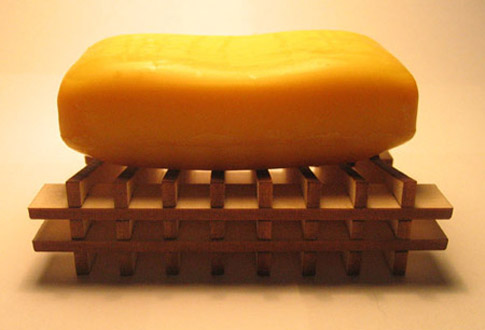
\includegraphics[width=0.4\linewidth]{img/flat-b.jpg}
}
\subfloat[] {
    \label{fig:laser-example-b}
    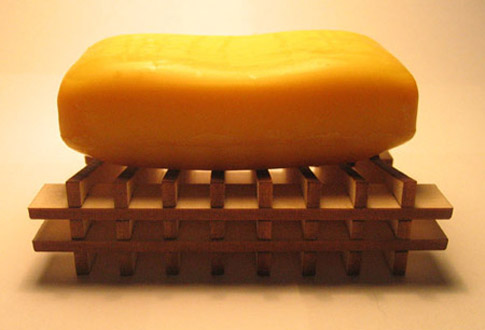
\includegraphics[width=0.4\linewidth]{img/flat-b.jpg}
}
\caption{Laser cut items.}
\label{fig:laser-example}
\end{figure}



Today, designers can choose among several modeling tools for laser
cutter projects. The most common is Adobe Illustrator, a
general-purpose, full-featured vector graphics editor. Mew users find
its interface familiar. Despite this sense of familiarity,
participants in our formative study (presented later) had a hard time
using Illustrator quickly and effectively. While Illustrator is a
powerful, feature-rich tool, it is intended primarily for graphic
design and does not provide support for the domain-specific activity
of designing for laser cutters. Experts use CAD tools such as Rhino or
SolidWorks that are perhaps more appropriate for this kind of
modeling, but also entail a substantial learning curve. If design by
avocational users is to become common, appropriate modeling tools must
be made available~\cite{lipson-homefactory}.

We present ``Sketch It, Make It'' (SIMI), a modeling tool for laser
cutter design based on recognizing short sequences of input sketched
with a stylus. Using only freehand drawn input, SIMI enables a
designer to iteratively and incrementally create precise laser cut
models.

Research on sketch-based modeling tools~\cite{johnson-sketch-review}
typically see sketching as an activity done mostly in the early phases
of design. Tools based on this assumption are justifiably oriented
towards capturing inprecise input while ignoring unimportant
detail. Only a few sketch-based systems support designers in later
stages when it is important to make decisions.

% TODO: Mark asked for citations for the above statement about
% sketch-based systems that support late-phase design. I could offer
% ParSketch, Lineogrammer, Furniture Factory, SketchChair, and maybe
% dig up whatever is going on with Igarashi/Lipson/Stahovich labs. But
% as far as I know, this is not a very strong statement, as nobody
% that I know of really has a system that supports both fabrication
% *AND* human-in-the-loop precision.

We are inspired by the potential of freehand drawing as a basis for
precision modeling for several reasons. Sketching is quick and can be
easily learned. It is simple and modeless: unlike structured editing
software, a designer need not set a pencil's mode to line, circle, or
anything else. Yet (as we shall show), a freehand sketch can provide
enough information to translate into a precise digital model.

\subsection{Contributions}

This paper offers four contributions: first we present the results of
a formative study on how people design objects for laser cutting. We
relate the process that avocational designers use and their
frustration with current structured modeling tools. We also provide an
analysis of artifacts from popular Maker community web sites that
reveal specific design features common to many laser cutter projects.

The primary contribution is \textit{Sketch It, Make It}, a tool
supporting iterative, incremental sketch-based modeling for designing
precise 2D shapes for laser cutting. Most prior work on sketch-based
modeling techniques explored specific topics (like corner finding,
recognition algorithms, or mode-switching). We improve on existing
sketch-based interaction techniques and bring them together in an
ensemble whose sum is greater than its parts. 

Last, we present the results of a user study of this tool. The
system's success depends on how well its individual features work well
together. We believe our system gives users a remarkably fluid
environment for designing laser cut items, a belief supported by this
study.

\section{BACKGROUND}

Laser cut designs are composed of parts cut from solid, flat pieces of
material and assembled in various ways: laminated, notched, bolted
together, \textit{etc}. The user can also design joints so the parts
fit together. Most joints have small margins of error. It is
imperative that lengths, angles, and relative position be indicated
precisely so that the parts fit together properly.

The designer's primary concern is to use the modeling tool to specify
outlines of parts to be laser cut. The modeling tool should output a
file using vector graphics to define part shapes, and raster images
indicating etching.

Many material types can be used, depending on the laser cutter. A
medium-sized machine has a cut bed supporting material about 18 by 24
inches (approx. 46 by 61 cm) and can cut through at most 3/8'' (1 cm)
soft wood. Common materials for cutting include wood, plastic,
leather, and paper. Different materials require different laser speed
and intensity settings to achieve a quality cut. Hard material like
metal can be etched on such machines. To cut through metal, a much
more powerful machine is needed. 

The laser leaves a gap in its wake, called a \textit{kerf}. The kerf
size depends on the speed and intensity of the laser. A typical laser
kerf is between about 0.2mm and 0.5mm on a 40 watt cutter. This is an
important consideration when designing facets whose tolerances are
small with respect to kerf. A notch joint, for example, is ineffective
if it is 0.1 mm too large or small.

The time to cut items depends on speed and intensity settings, and on
the size and complexity of the cut path. For example, the assembly
shown in~Figure\ref{fig:TODO} took about five minutes to fabricate and
used about \$3.50 (2012 USD) in material. 

% unlike some other past tools in sketching, precision is paramount
% here (explain why). This argument should go either here or when SIMI
% is first introduced in depth.

\section{RELATED WORK}

While ``the design process'' has important differences between
domains, two properties are common to many types of modern design
work, including design for laser cutters. First, designers sketch
throughout the process, especially at the outset. Second, a computer
tool is used to render the design more precisely. The properties are
confirmed by observations of graphic
designers~\cite{wong-rr-prototypes}, automotive
engineers~\cite{kara-styling}, and software
developers~\cite{dekel-improvised-notation}. Freehand drawing is a
powerful means for thinking and specifying design intent, but as many
have observed, it is disconnected from the computer aided portion of
the design process~\cite{company-sketching-in-engineering}.

\subsection{Sketch-based interaction}

The rough appearance of freehand sketches encourages designers to see
beyond unimportant details, letting them make big-picture
decisions. Much prior work argues that rectification is antagonistic
to design~\cite{gross-cocktail}, at least during the conceptual
phases. One system that takes this perspective is SILK. It is a
sketch-based tool for quickly drawing user
interfaces~\cite{landay-silk-chi}. It recognizes user input as UI
elements like menus, scrollbars or buttons and transforms the
recognized sketch to a working implementation, while retaining its
rough appearance.

% So: SILK throws it over the wall when conceptual design is done,
% expecting the designer to finish the job in code (e.g. how does one
% set the exact pixel alignment or padding if not in code?) SIMI lets
% users give precise details without the need for help from grown-up
% tools.

Some work takes an alternate view on the appearance of sketched
input. Systems such as Pegasus~\cite{igarashi-pegasus} and recent work
by Murugappan \textit{et. al}~\cite{murugappan-beautification}
`beautify' the drawing by replacing rough input with cleaned-up
graphic elements like lines or arcs. These 2D graphics systems infer
the user's intention by inferring geometric relationships. If more
than one relationship is possible, the system lets the user choose
among a small number of alternatives. These tools enable users to
quickly and easily make clean-looking vector graphics. However, the
aggressive inferencing can make it difficult to make drawings that
have subtle features the system can not infer.

% So: While inferencing is powerful, it also prevents one from making
% subtle distinctions. E.g. the designer wants a circle *near* a line
% but not tangent to it. SIMI enables this level of control.

Sketch input is an appealing way to interact with computers because
users find it natural and easy to provide. Unfortunately, sketch
recognizers are not yet sophisticated enough to reliably interpret
arbitrary drawings. Therefore researchers have created ways to close
the gap between input that people would like to provide and the
computer's ability to make sense of it. For example a system may
require users to draw in certain ways (e.g. shapes must be drawn with
single strokes) to conform to the recognizer's capabilities, as in
SILK. 

Teddy~\cite{igarashi-teddy}, EverybodyLovesSketch~\cite{bae-everybody}
are among those that develop or refine sketch-based interaction
techniques that that are both natural for humans to use and easier for
the computer to understand.  They provide a small grammar of
easy-to-use gestures that people use to create and edit 3D
drawings. The ease and power of these systems is evident: children can
learn and use them to make complex models. EverybodyLovesSketch in
particular seeks to enable a broad audience to create 3D perspective
conceptual sketches by choosing a set of gestures and tools that work
well together. Despite their power, however, it is hard to engineer
with these tools because they do not provide users the ability to give
dimensions to arbitrary lengths or angles. SIMI builds on the 

% So: power and ease of use are not mutually exclusive, but it
% requires careful tuning of interaction techniques to make it
% work. SIMI builds on this.

\subsection{Sketch-based modeling for fabrication}

Computer support for fabrication design has been a topic of interest
for decades, under the rubric of computer aided design (CAD) and
computer aided manufacturing (CAM). While today interaction is mostly
performed with a keyboard and mouse, this was not always the case. For
example, SketchPad~\cite{sutherland-sketchpad} users controlled the
design by setting modes and parameters using one hand while drawing on
the screen with a light pen in the other.

More recently, novel interfaces enable users to model items for
fabrication by sketching. For example, people can use
Plushie~\cite{mori-plushie} to design soft objects such as stuffed
animals. Users begin by creating 3D models of bulbous objects by
sketching in a manner similar to Teddy~\cite{igarashi-teddy}. The
program outputs a set of 2D shapes that users can cut from fabric,
sew, and stuff.

Sketch Chair makes design for rapid fabrication more
accessible~\cite{saul-sketch-chair}. Users sketch the contours of a
chair's seat and back rest, and (in a different drawing mode) add
legs. It also allows designers to change subtle properties of curves
using on-screen control handles.  The system includes a sophisticated
physical simulator to let the designer explore design consequences
(for example to determine if it will remain upright).

Domain-oriented tools such as Plushie and Sketch Chair enable people
to make things they otherwise would be unable to, but the designer
relinquishes a great deal of control to the system. In contrast, SIMI
users retain the ability to specify as much or as little as they like
at the expense of domain-specific assistance.

SIMI builds on the work of a fairly small but interesting set of
sketch-based systems that support precision. With
ParSketch~\cite{naya-parsketch} designers create parametric 2D models
by incrementally recognizing sketched geometry and commands. It uses
pressure to distinguish between linework (high pressure) and
constraint commands (lower pressure). Lineogrammer is a sketch-based
2D drawing tool that lets users make rectified vector graphics. Like
Pegasus~\cite{igarashi-pegasus}, it works on the principle of
interactive beautification, supporting iterative sketch/rectify
sequences. The interactive nature of these precision-oriented systems
means the system has less work to do when its recognizer/rectifier is
invoked. This generally leads to more accurate recognition and higher
user satisfaction.

% TODO: someone wants me to support the bit about smaller batches
% leading to more accurate recognition and higher
% satisfaction. Actually I'm not sure I can find anybody who has
% dwelled on this because it seems obvious: given a choice of five
% things, it is clear that I will pick the right one more often than
% if I am given a choice of a thousand things.

\section{BACKGROUND STUDY}

To better understand the design and development practices involved
with laser cutter fabrication we conducted two related empirical
studies. We interviewed people with experience designing these
artifacts, and watched them work. We also surveyed and analyzed
laser-cut items on community web sites to find common features. These
studies were conducted to help us better understand the kinds of tasks
and problems designers face when designing for laser cutters, which in
turn informed development on SIMI.

\subsection{Formative Study on Designer Work Practices}
\label{sec:formative}

We interviewed six designers to learn about their work practices and
to understand how they use their tools. All participants had
substantially different backgrounds, including mechanical engineering,
graphic design, and architecture.  They were experienced with
designing for and using laser cutters. The participants were part of
our tool's target demographic: people who make (or want to make)
things with laser cutters as a hobby.

Each session lasted approximately an hour and was split evenly between
interview and implementation. We met participants in their own work
environments (offices or labs). Participants were to describe their
design process, and to show sketches or videos of their work. While
there are differences (some subtle) in their process, each followed
the same overall pattern.

They all begin by thinking about a problem and sketching. Some
sketches were are made to think about how to frame the project (what
it is for), whereas others help reason about how to make it (how it
works, how it fits together). Some designers explicitly noted that
sketching is a necessary part of the process, stating that it would be
impossible to move forward without making freehand drawings. Only
after the idea is reasonably well-formed they will translate their
hand-made sketch into a computer model (Figure~\ref{fig:translate}).

\begin{figure}[h]
  \centering
  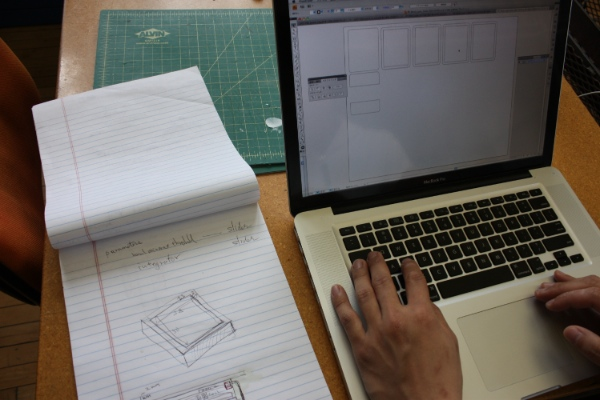
\includegraphics[width=0.9\linewidth]{img/translate-sketch-to-computer.jpg}
  \caption{A common part of designing for laser cutters: translating a
    hand-made sketch to a computer modeling tool. The sketch includes
    a perspective drawing of the desired result, and 2D diagrams of
    individual parts with key dimensions indicated.}
  \label{fig:translate}
\end{figure}

After the work practices interview, we asked participants to implement
the sketch shown in Figure~\ref{fig:interview-sketch} using a software
tool of their choice. Our purpose was to learn what problems
people encountered when executing the common task of translating a
sketch to a computer model.

\begin{figure}[h]
\centering 
\subfloat[The part users set out to replicate.] {
  \label{fig:interview-sketch-1} 
  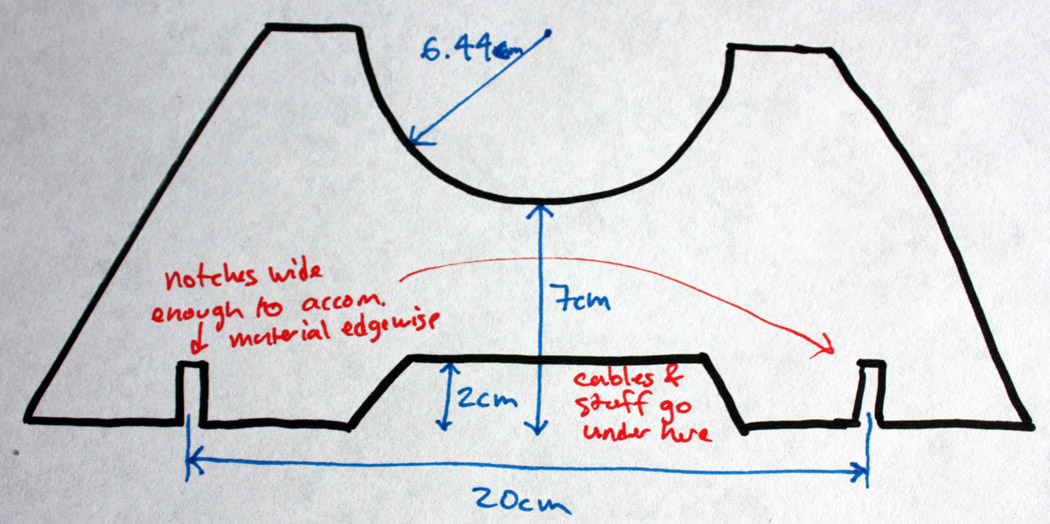
\includegraphics[width=0.9\linewidth]{img/laser-me-1.jpg}
}

\subfloat[Drawing of how the part is used in context.] {
    \label{fig:interview-sketch-2}
    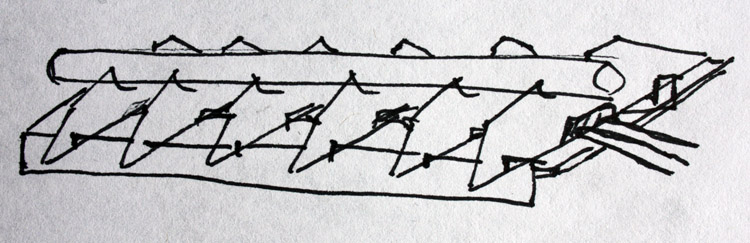
\includegraphics[width=0.9\linewidth]{img/laser-me-2.jpg}
}
\caption{Participants were asked to create the stencil at the top
  using modeling software.}
\label{fig:interview-sketch}
\end{figure}

Most participants chose to implement the sketch with Illustrator (5
users); one chose Rhino. In every case, the designer's strategy
involved common activities: creating or editing boundaries, aligning
or snapping items, using guide lines or reference points, measuring
distances, specifying or changing lengths and angles, and creating
finished ``cut files'' to send to the laser cutter.  They also engaged
in the usual interaction management tasks such as
selecting/deselecting on-screen elements, or view port management like
zooming and panning.

Participants spent a good deal of time on operating overhead
(approximately 50\%)---(1) searching for the appropriate tool for the
next task, (2) recovering from errors made after selecting the wrong
tool, or (3) when the tool behavior was inconsistent with the user's
intention.

For example, one user was aware of Illustrator's ``Path Finder'' tool
and wanted to use it. The user searched the program's menu structure
and hovered over toolbar buttons to read tool tips before finding
it. Next, the designer invoked various functions of the Path Finder,
using the keyboard shortcut to undo after each failed attempt, as he
searched for the correct mode within the subcommand palette. This
process lasted approximately 80 seconds before finally being able to
continue. This person has used Illustrator for several years and could
not be considered a new user.

Occasionally participants used features in rather strange ways to
achieve a desired outcome. For example, in order to remove an unwanted
segment of a polyline, one participant (a graphic designer) created an
opaque white rectangle to obscure it, rather than erase it. (``Don't
tell anyone I did this'', he said at the time).

Similar episodes are common: a person \textit{should} know the
`correct' action, but takes an alternate approach. The alternative
might achieve the intended effect, but it might be less efficient
(more operations, longer execution time) or it might introduce
unwanted complexity (such as the invisible white rectangle).

To summarize, we found most common tasks and problems found in
interview study and formed three main groups:

\begin{itemize}
\item \textit{Defining geometry:} Creating/editing boundaries,
  aligning items, creating and using guide lines or reference points,
  measuring distances, and specifying lengths or angles.
\item \textit{Managing the editing tool:} Selecting/deselecting
  objects, view port management, finding and entering tool modes, and
  recovering from errors.
\item \textit{Cutfile:} Finalizing the cutfile by creating copies of
  items when more than one is needed, and positioning stencils.
\end{itemize}

\subsection{Artifact Analysis}

To learn more about the characteristics of laser-cut assemblies made
by DIY makers, we analyzed finished items from two web-based
communities. Together with the study on how people make items, this
helps inform development of SIMI.

Many users are motivated by the opportunity to share their designs
with others. Ponoko and Thingiverse are two currently popular web
sites for selling or sharing items that can be made with rapid
fabrication machines. Ponoko offers thousands of user-designed items
for sale, most of which are produced with laser cutters. Thingiverse
is a warehouse of digital models that mostly contains 3D-printable
objects but also includes many designs for laser cutters. From these
two sites we selected a total of 55 laser-cut projects. On Ponoko we
selected the first 45 items that were made with laser cutters. On
Thingiverse we searched for objects with the ``laser cutter'' tag. We
then examined the features of these 55 projects to better understand
what people are making with laser cutters. The results of this
analysis are summarized in Figure~\ref{fig:ponoko}.

\begin{figure}[h]
  \centering
  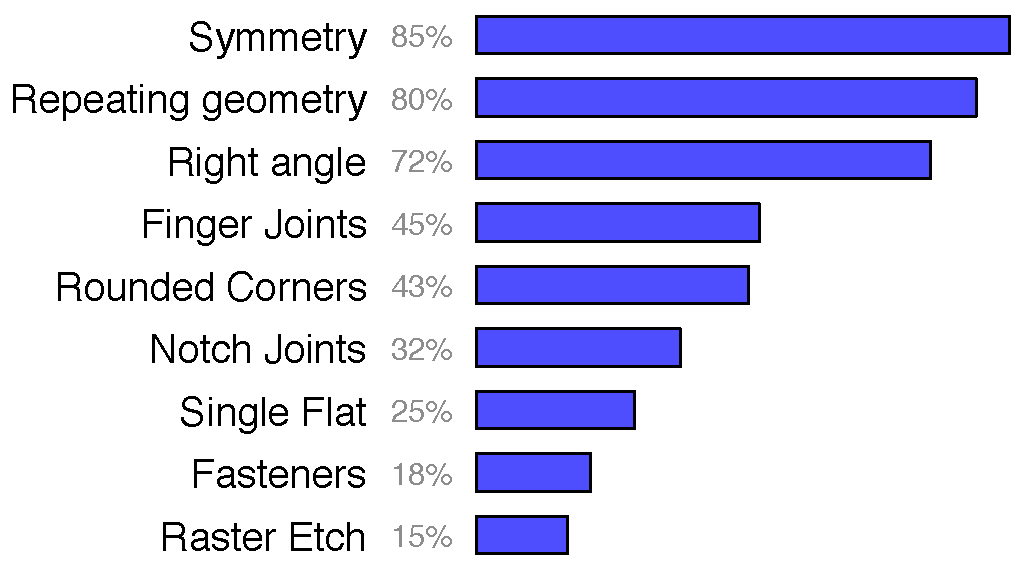
\includegraphics[width=0.9\linewidth]{img/ponoko-graph.pdf}
  \caption{Frequency of certain features present in 55 laser-cut
    designs found on Ponoko and Thingiverse.}
  \label{fig:ponoko}
\end{figure}

We used nine properties to characterize each project, based on our own
experience designing objects for laser cutters, as well as from
observations from the formative study. These properties are summarized
here and described in greater detail below:

\begin{itemize}
\item \textit{Right Angle}: Edges meet at 90-degree angles.
\item \textit{Notch and Finger Joints}: Two parts come together using one of
  the joints illustrated in Figure~\ref{fig:joint}.
\item \textit{Single part}: Project is composed of a single, flat piece of
  material (e.g. a coaster).
\item \textit{Fasteners}: Clear use of glue, screws, or bolts.
\item \textit{Symmetry}: Radial or linear symmetry is a dominant feature.
\item \textit{Rounded Corners}: Right-angle corners are slightly blunt.
\item \textit{Raster etch}: Laser cutter etched patterns (e.g. words,
  images) rather than cutting all the way through material.
\item \textit{Repeating geometry}: Linework is repeated several times,
  often in a way that suggests procedural generation.
\end{itemize}

\begin{figure}[h]
\centering 
\subfloat[Notch joints.] {
  \label{fig:joint-notch} 
  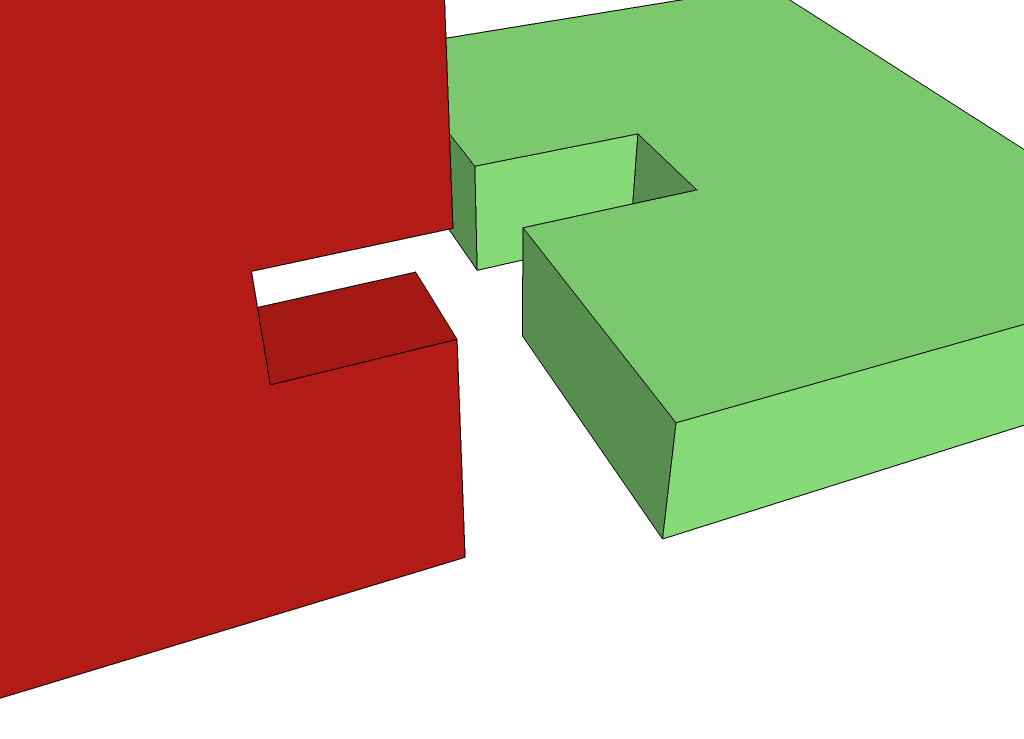
\includegraphics[width=0.4\linewidth]{img/joint-notch.png}
}
\subfloat[Finger (box) joints.] {
    \label{fig:joint-finger}
    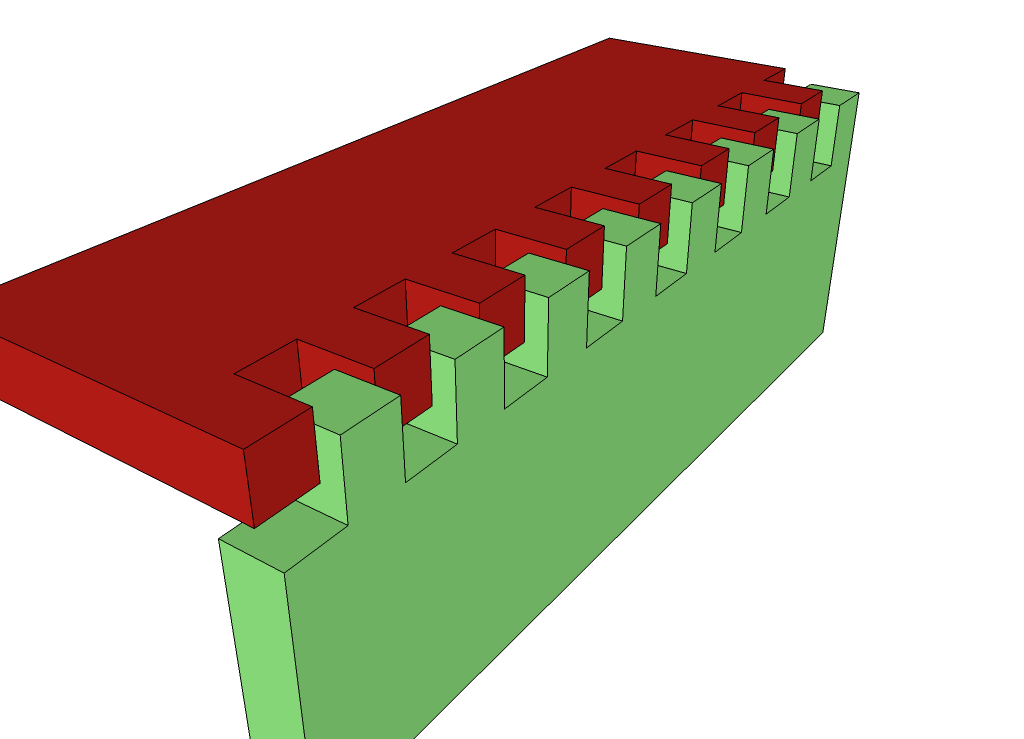
\includegraphics[width=0.4\linewidth]{img/joint-finger.png}
}
\caption{Two common methods to join parts. Notch joints are used when
  parts intersect along part midsections; finger joints (alternately
  called box joints) join parts along edges.}
\label{fig:joint}
\end{figure}

Single part projects were typically artistic, using expressive, curvy
linework. Among multi-part objects, approximately 75\% used finger or
notch joints (Fig.~\ref{fig:joint}). The rest used fasteners.

The more professional-looking models were those that used rounded
corners. Several designs used raster etching for artistic
effect. Repeating geometry was found in most models. These patterns
involve sequences of lines or curves with consistent length and
angles. Some patterns were quite ornate.

\section{SKETCH IT, MAKE IT}

Based on observing designer's work practices and the artifacts they
make, we developed \textit{Sketch It, Make It} (SIMI), a sketch-based
tool for modeling laser cut items. We aim to address problems with
current modeling systems enumerated above in a tool that specifically
supports designing laser-cut items.

Design for laser cutting requires precision. The greatest distinction
between SIMI and prior sketch-based desgin tools is its ability to
give users the ability to accurately specify geometry. That is, the
user may change lengths, distances, or angles by arbitrarily small (or
large) values. But in keeping with the spirit of sketch-based
modelling, the user is not obliged to give details if they are not
important.

%% The focus of this work is to produce a useful and usable sketch-based
%% design tool for the domain of laser cutting. The main challenge in
%% achieving this was the lack of a set of interaction sketch-based
%% techniques that work in harmony. Prior work has focused largely on
%% individual techniques that clearly map problems to solutions. In
%% contrast, our system address the challenge of developing a system that
%% integrates many experimental interaction techniques into a coherent
%% whole.

SIMI users draw with a stylus, using and an offhand button for a few
actions. The system recognizes input as either geometric linework or
gestural commands. Linework includes straight lines, elliptical arcs,
splines, circles, and ellipses.

Users invoke commands to operate on linework by drawing gestures. Some
gestures are recognized and execute immediately, such as the erase
(scribble) gesture. Others, such as a command to constrain segments to
be the same length, are recognized after the user presses the button,
or after a timeout.

The system recognizes a closed 2D path as a `stencil'. Stencils are
shapes that can be placed on the virtual laser cutter bed. Several
copies of a stencil can be added. The system generates a vector file
that can be sent directly to a laser cutter.

After cutting stencils, the user assembles them to their final
configuration. Figure~\ref{fig:laser-example} shows examples of
projects made with SIMI.

\subsection{Sketch Interaction Techniques}

\begin{figure}[h]
\centering \subfloat[Automatic: merge when endcaps intersect
  (drawn in blue).] {
  \label{fig:latch-auto} 
  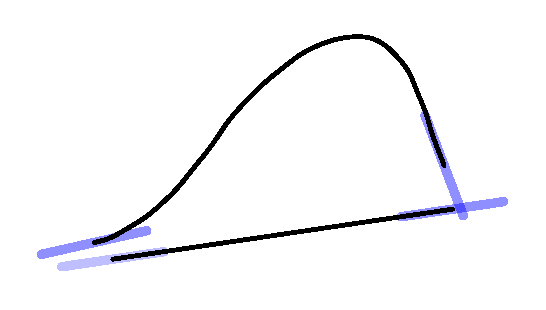
\includegraphics[width=0.43\linewidth]{img/latch-auto-endcaps.pdf}
}\hspace{5mm}
\subfloat[Latching endpoints.] {
  \label{fig:latch-endpoint} 
  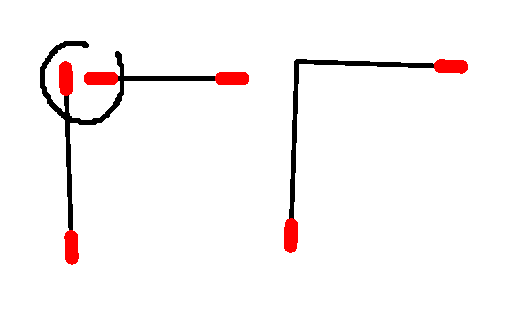
\includegraphics[width=0.43\linewidth]{img/latch-manual-endpoint.pdf}
}
\\
\subfloat[Latching continuation.] {
    \label{fig:latch-continuation}
    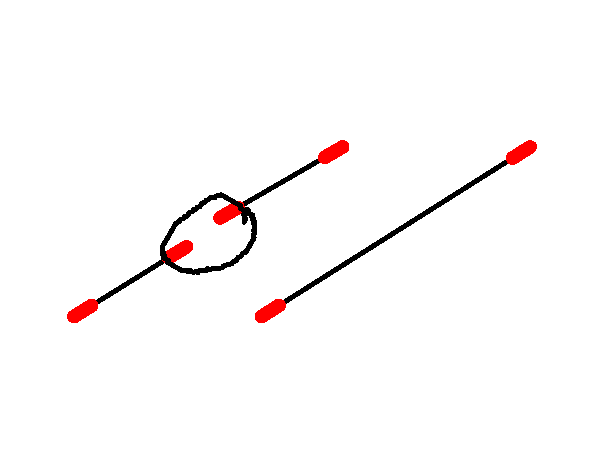
\includegraphics[width=0.43\linewidth]{img/latch-manual-continuation.pdf}
}\hspace{5mm}
\subfloat[Latching T-Junction.] {
    \label{fig:latch-tjunct}
    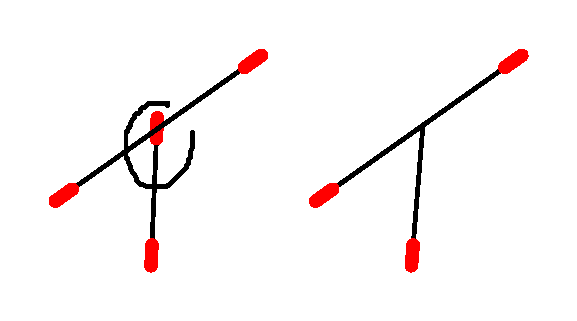
\includegraphics[width=0.43\linewidth]{img/latch-manual-tjunct.pdf}
}
\caption{Automatic and manual latching used to bring segments together.}
\label{fig:latch}
\end{figure}


%* Stylus with offhand button

Guiding the development of SIMI is the principle that the designer
should never need to set down the pen. Input is provided entirely with
a stylus except for a single button used by the non-dominant hand that
gives access to additional commands. The gestures used to invoke
commands or add constraints are summarized below.

\subsubsection{Latching}

Users often want adjacent lines to meet at a common point. In the user
evaluation designers struggle to make lines coterminate. Sometimes the
designer would simply extend the lines past each other to ensure the
laser path will make the corner correctly. 

Latching is the process of combining adjacent segments (lines,
splines, arcs, \textit{etc.}) so they meet at a common point. For
example, users may draw a square with with four strokes, and eight
unique end points, but a square should have only four corners.

SIMI provides two methods for latching segments, illustrated in
Figure~\ref{fig:latch}. One is automatic: the system analyzes new
linework for cases where the user probably meant their segments to
join together, and adjusts one or more segments to join. Automatic
latching can be problematic if it is too zealous. Early approaches
used only distance to find which segments should be
latched~\cite{herot-latch-corners}: if two endpoints were within $x$
units of one another, latch them. This works well when segment lengths
are large relative to $x$. But when the segments are short, a naive
latcher merges points that the designer intended to remain distinct.

SIMI's automatic latcher uses length and the segment direction at the
endpoint. It creates an \textit{endcap}: a short line segment centered
at an end point that extends the line by a fraction of its length
(currently 0.1). For nearby segments to latch automatically, their
endcaps must intersect. SIMI can latch two or more segments this way.

The automatic latching process is intentionally conservative to avoid
frustrating users. Therefore it often misses cases where the user
wanted lines to meet. SIMI gives users a simple method to latch
segments: draw a small circle around the endpoints to be latched.

All linework in SIMI is meant to compose stencils, which are sequences
of latched segments. Therefore the designer must be able to find and
fix un-latched segments. The system draws a red marker at lonely
endpoints to reveal un-latched segments.

Three different spatial arrangements can be latched: endpoint
latching, continuation, and T-junctions (see
Figure~\ref{fig:latch}). Endpoint latching is what the automatic
latcher does. Continuation latching is when the user brings together
two segments that are close to the same direction at the joined
point. Continuation latching replaces two segments with a single
larger segment. A T-junction is when a segment endpoint latches to the
middle of another segment, splitting the second segment in two.

\subsubsection{Erase}

\begin{figure}[h]
  \centering
  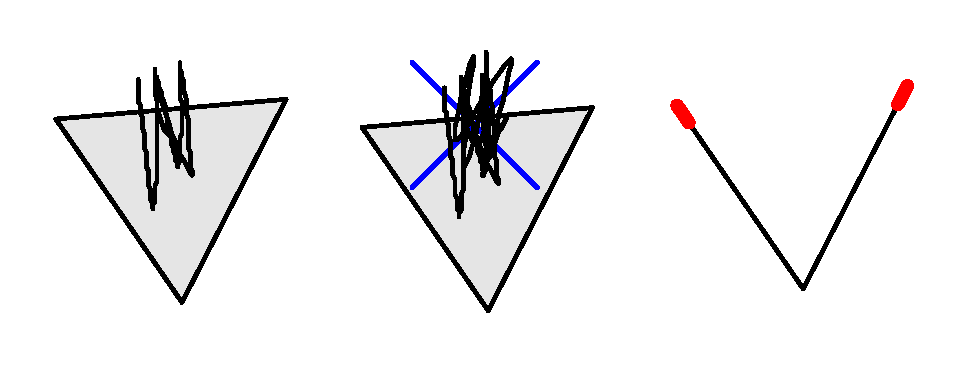
\includegraphics[width=0.9\linewidth]{img/erase-all.pdf}
  \caption{Erase gesture: before, during, and after.}
  \label{fig:erase}
\end{figure}

Users may want to remove linework for various reasons: deleting
unwanted or accidental items, or as part of a deliberate strategy to
cut away geometry to allow new shapes to
emerge~\cite{zeleznik-lineogrammer}. Like latching, erasing is a
common task so it is invoked with a simple scribble gesture. During
development we tried various algorithms for detecting the
scribble. The first attempts were computationally intensive enough
that they could only be performed once after the pen was
released. However, test users found it difficult to perform the
gesture correctly. Worse, when done incorrectly the input would be
recognized as linework and remain on the canvas. This raises another
need to erase using the same problematic algorithm. This caused
considerable frustration.

Our new algorithm for detecting erasure executes efficiently during
the pen stroke. When an erasure gesture is detected mid-stroke, it
provides visual feedback that gives users confidence and avoids
frustration. Figure~\ref{fig:erase} shows an erase gesture with the
visual feedback.

Erase (scribble) gestures are detected as follows. First we assign
each point $P_i$ with a time stamp $T_i$, a curvilinear distance
$D_i$, and a heading vector $H_i$. Curvilinear distance is the path
length along the stroke from the first point: $D_0=0$, and the
rest are $D_i = D_{i-1} + distance(P_{i-1}, P_i)$.

A pen stroke is not considered an erasure if the pen has moved less
than a minimum distance from the start point (we use 10 pixels).

The heading $H_i$ is a normalized vector from $P_{i-k}$ to $P_{i+k}$,
for a window size of some $k$ (we use $k=1$ but for higher resolution
input surfaces $k$ should be larger). The first $k$ points use $H_k$
for their heading.

Next we add points to a list of samples $S$. If $D_i$ is more than
some threshold beyond the most recently added sample point, $P_i$ is
added to $S$. When a new sample point is added, it assembles a
sub-list $R$ of recent sample points that occurred within $t$
milliseconds (our implementation uses 100ms). If the angle between any
point in $R$ and the new point is greater than some value (we use
$\pi$ radians), it increments a `corner' count value for the current
pen stroke. When enough corners are found (we use 5) for a stroke, the
system draws feedback to alert the user that the gesture has been
recognized and halts recognition until the pen is lifted.

Because the sample list depends on a relatively short duration, the
user must scribble vigorously to activate the erase gesture. The user
who intends to erase but draws slowly, quickly learns to scribble a
little faster and wait for the visual feedback.

\subsubsection{Undo and Redo}

Participants in our designer evaluation used the feature in two
distinct ways: to revert state following epistemic actions and
usability problems~\cite{akers-undo}. First, the Undo function gives
designers confidence to modify their work to see what changes might
look like. These epistemic actions~\cite{kirsch-epistemic-action}
support creative exploration. If the designer does not like their
modifications they simply Undo to a prior state. The second class of
Undo events stems from errors: either usability problems or user
error. Regardless of the reason for invoking Undo, it is clearly a
useful feature. 

Users undo by holding down the offhand button and dragging the pen to
the left. Every 40 pixels left triggers one undo action. This lets the
designer undo several actions by simply dragging farther to the
left. Redo is done by dragging to the right. Both undo and redo
actions can be triggered by the same stroke by changing
direction. This lets the designer scan for a desired state by dragging
left and right.

\subsubsection{Right Angle and Length Constraints}

Most laser cut stencils employ right angles, symmetry, and repeated
geometry (see Figure~\ref{fig:ponoko}). Designers can create stencils
that have these properties by imposing geometric constraints. A
constraint is a rule that enforces some mathematical property, usually
in the form of a geometric relationship among two or more
elements.

\begin{figure}[h]
  \centering
  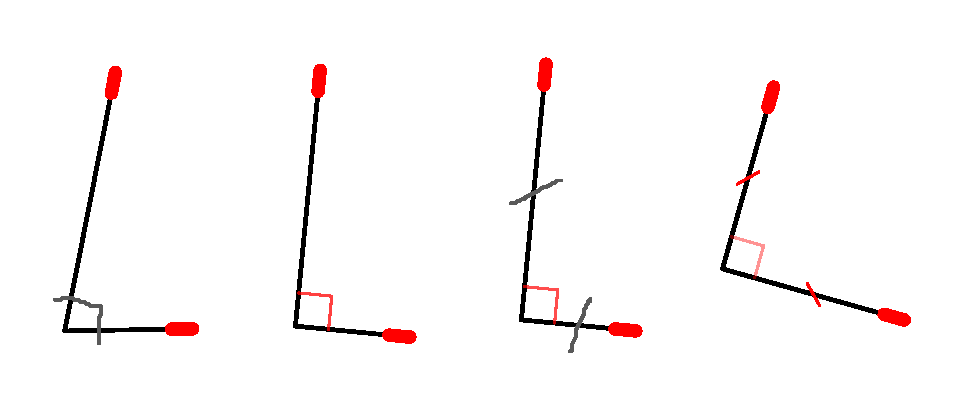
\includegraphics[width=0.9\linewidth]{img/constraints-all.pdf}
  \caption{Gestures for adding a right angle (left) and same-length.}
  \label{fig:constraints}
\end{figure}

In SIMI, designers add constraints with drawn gestures. In traditional
drafting and standard geometry diagrams, a brace symbol at the
intersection of the two edges indicates a right angle. SIMI recognizes
drawn input that looks like that brace and adds a constraint on the
associated segments. These are shown in
Figure~\ref{fig:constraints}. Erasing either segment in a right-angle
constraint also removes the constraint.

Another drafting convention uses tick marks (hash marks) to indicate
that two lines are the same length. SIMI recognizes two or more ticks
crossing line segments as a gesture to create a \textit{same length
  constraint}. A same-length constraint is satisfied when all segment
lengths are equal. The target length is the mean value of the
constituent lengths.

SIMI also lets designers set specific lengths, invoked by selecting a
line (by over-tracing a portion of it) and typing a
number. (Handwriting recognition would be preferred.) If one of the
segments in a same-length constraint is assigned a particular length,
all segments take on that particular length.

\subsubsection{Flow Selection}

% Justify wrt user study and Ponoko analysis

About a third of the models we looked at in our Ponoko analysis
involved curves that are typically modeled using splines (e.g. Bezier
curves). SIMI provides Flow Selection~\cite{johnson-flow-selection}
that enables users to manipulate create and modify splines
(Figure~\ref{fig:fs}). The user `heats up' portions of curved segments
by holding the pen down near the curve. Then, without picking the pen
up, the user deforms the heated region by dragging the pen. ``Hotter''
points along the curve move more.

\begin{figure}[h]
\centering \subfloat[Selecting (``heating'') points along a curve near
  the stylus. The selection grows as long as the stylus is held down. ] {
  \label{fig:fs-1} 
  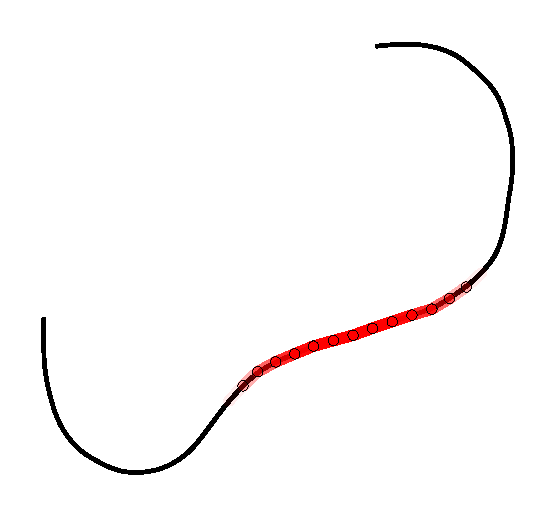
\includegraphics[width=0.4\linewidth]{img/fs-1.pdf} }
\hspace{3mm} \subfloat[Deforming the region by moving the
  stylus. ``Hotter'' points (close to the pen) are moved more than
  those farther away.] {
  \label{fig:fs-2} 
  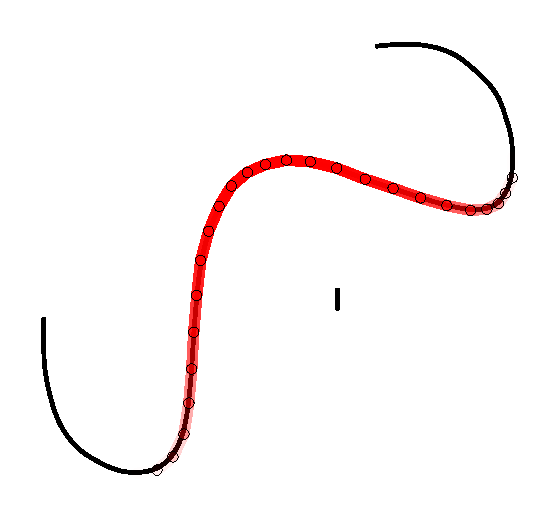
\includegraphics[width=0.4\linewidth]{img/fs-2.pdf}
}
\caption{Flow selection.}
\label{fig:fs}
\end{figure}

% TODO: add to flow selection section.

\subsubsection{Reference Points and Guides}

% Justify wrt user study and Ponoko analysis

In our study on designers, we noticed people measuring distances and
drawing temporary lines used to anchor subsequent linework. For
example, the stencil illustrated in
Figure~\ref{fig:interview-sketch-1} calls for a semi-circular region
in the middle of the top edge. Participants noted that their preferred
strategy for making this stencil was to draw a long line along the
top, and add the circular region afterwards. However, none of the
Illustrator users were able to successfully take this strategy because
they did not know how to find the midpoint of the line. Instead of
carrying out their desired plan they measured the distance of the top,
and added co-linear lines with half the length that met in the
middle. This was an error-prone and time-consuming process. To support
strategies like the one mentioned above, SIMI gives users the ability
to use reference points and guides.

\begin{figure}[h]
  \centering
  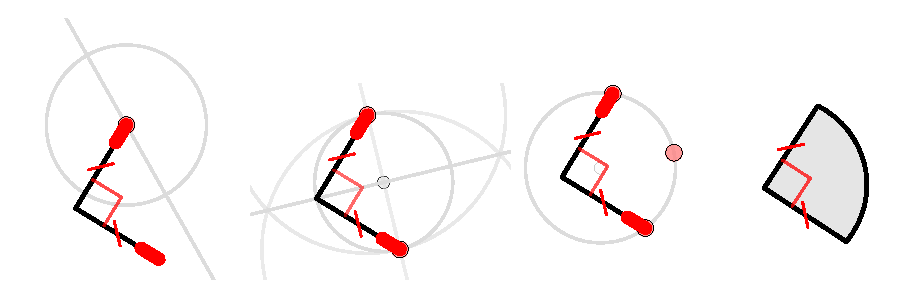
\includegraphics[width=0.9\linewidth]{img/guides-all.pdf}
  \caption{Reference points and guides. The first three panels show
    one, two, and three reference points and the guides that are
    displayed as a result. The designer uses the circular guide to
    create the circular arc shown in the final panel.}
  \label{fig:guides}
\end{figure}

The user may create handles to move segment endpoints around by
drawing `reference points'. These are dots made by swirling the pen
around in a tiny area (within 9 pixels) quickly (less than 500ms). The
user can then reposition the reference points to adjust attached
geometry by dragging them.

When reference points are present, the system offers guides to aid
additional drawing. The possible combinations are illustrated in
Figure~\ref{fig:guides}. When there is one reference point, the system
uses the pen's hover location, drawing a circle centered at the
reference point, and a line passing through both. This can be used to
make a hole centered at a particular location.

Two reference points give the user three circles, two lines, and shows
the midpoint. Three reference points give the user a circle that
passes through them, and indicates that circle's center.

\subsection{Constraint Engine}

SIMI lets designers establish \textit{constraints} that enforce
geometric relationships among items~\cite{borning-thinglab}. For
example, the user might draw a triangle and establish a right angle
constraint. No matter how the user manipulates the drawing (moving
vertices or changing segment lengths), the constraint engine maintains
that particular corner as a right angle.

SIMI's iterative, numeric solver minimizes the total error of all
constraints. A constraint's error is computed as how far each related
point must move to satisfy the constraint. However, a point may be
involved in several constraints, so it is not generally possible to
simply move points to where they satisfy one constraint because it
might break one or more other constraints. To manage contending
constraints, the system computes a change vector for each point by
computing the change required by all related constraints. Each point
moves a small amount along its change vector, and the process
continues until the total error becomes minuscule.

The solver can get trapped in a loop as points oscillate between
several values. We use simulated annealing~\cite{metropolis-annealing}
to avoid this case: the amount that points move varies randomly, and
is larger when there is more entropy. Gradually the system reduces the
level of randomness and the points settle in to a satisfactory
configuration.

\subsection{Stencils}

SIMI's final product is a ``cut file'': a vector drawing for a laser
cutter. This cut file typically contains a number of stencils, which
are closed 2D shapes that define the laser's path. Stencils may have
complex boundary geometry with non-intersecting edges. Stencils can
also have any number of holes in them, for joints, fasteners, or other
purposes.

To identify stencils, SIMI forms a graph with segments as edges and
their endpoints as nodes. It then runs a depth-first search. Cycles
from a given point is a candidate stencil. After completing the
search, only the longest paths are kept. Stencils are visually
represented by shading the interior.

\section{EVALUATION}

* screenshots/photos from user study

* other results from user study...

\section{FUTURE WORK}

Future work...

\section{ACKNOWLEDGMENTS}

% TODO: fill this in later. Leave left blank for blind review.

For those about to rock, we salute you.


\bibliography{simi}

\end{document}
